\chapter{Time-of-Flight Signatures of Bosons in a Double Well}
\index{Appendix!Time-of-Flight Signatures of Bosons in a Double Well@\emph{Time-of-Flight Signatures of Bosons in a Double Well}}%
\label{appendix-tof}
%
\section{Introduction}
The main text of the dissertation details how a two-boson system can be subjected to a micrometer-scale double well by various means. Ensembles of such systems can also be generated. For optical systems, an optical lattice of such double-wells can be generated by two counter-propagating lasers of linearly polarized light with a known angle between their planes of polarization, and a transverse magnetic field to mix the two potentials~\cite{Deutsch:Jessen}. If the on-site lattice depth is sufficiently deep then the tunneling between the sites can be neglected. For magnetically confined systems, such an ensemble can be generated by repeated measurements.

In the following sections, we evaluate the time of flight (tof) signatures of these wavefunctions, and discuss the extent to which they are useful in distinguishing the different outcomes of STIRAP, depending on the rate at which the time modulated radiation pulses sweep across the Floquet eigenphases. The presence of extra avoided crossings due to broken symmetries affect the outcome of STIRAP by changing the final eigenstate of the system. This will change the number of oscillations seen in the tof distribution. These oscillations can be resolved by choosing an appropriately high value of the time of flight $\tau$ which reduces the frequencies. The momentum probability distributions of the tof do not provide enough information to uniquely profile the original wavefunction spatially, since two neighboring states with opposite parities will provide nearly the same tof distribution. However, quantum control methods like STIRAP can be tuned to forbid those transitions, making tof a valuable tool in profiling the final states of quantum controlled excitations in cold atom systems. 

Section~\ref{sec:1:appendixtof} will elaborate on the regions of interest in the parameter space of this problem. In section~\ref{sec:2:appendixtof}, we will discuss the nature of the time-of-flight signatures of the different states. Numerical results will be shown in section~\ref{sec:3:appendixtof}. 


\section{\label{sec:1:appendixtof} The Strongly Interacting and Single Particle Regimes} 
%
%
The total Hamiltonian for the 2-boson system is again,
\begin{equation}
H =p^2_1+p^2_2+V_0 (-2 x_1^2+ x_1^4) +V_0 (-2 x_2^2+ x_2^4)+U_0 \delta(x_1-x_2) .
\label{eq:hamscale:appendixtof}
\end{equation}
We will investigate the tof distributions in two regimes of the $\left(V_0,U_0\right)$ parameter space of the double well system. Here, $V_0$ is the well depth, and $U_0$ the amplitude of the point contact pseudopotential in 1-dimension.
The first regime, henceforth referred to as the 'strongly interacting regime' will consist of a very strongly repulsive system and a moderate well depth. We define the 'strongly interacting factor' for this system, $\gamma$, as 
\begin{equation}
\gamma \equiv \frac{U_0}{E}.
\end{equation}
Here, $E$, the energy of the state, is a measure of the ability of the bosons to tunnel across from one well to another. When $\gamma \rightarrow \infty$, we reach the strongly interacting regime where the interaction completely dominates the system~\cite{tonks:gas}. Figure~\ref{fig:tonksparam:appendixtof} shows the evolution of the ground state of the system as $\gamma$ is increased. The order parameter being plotted as a function of $\gamma$ for the ground state is $p_i/{\delta l}$, where 
\begin{equation}
p_i \equiv \delta l \int dx| \langle x , x | E_1 \rangle |^2.
\end{equation}

%Fig. 2
\begin{figure}
\hspace*{-0.2in}
\ 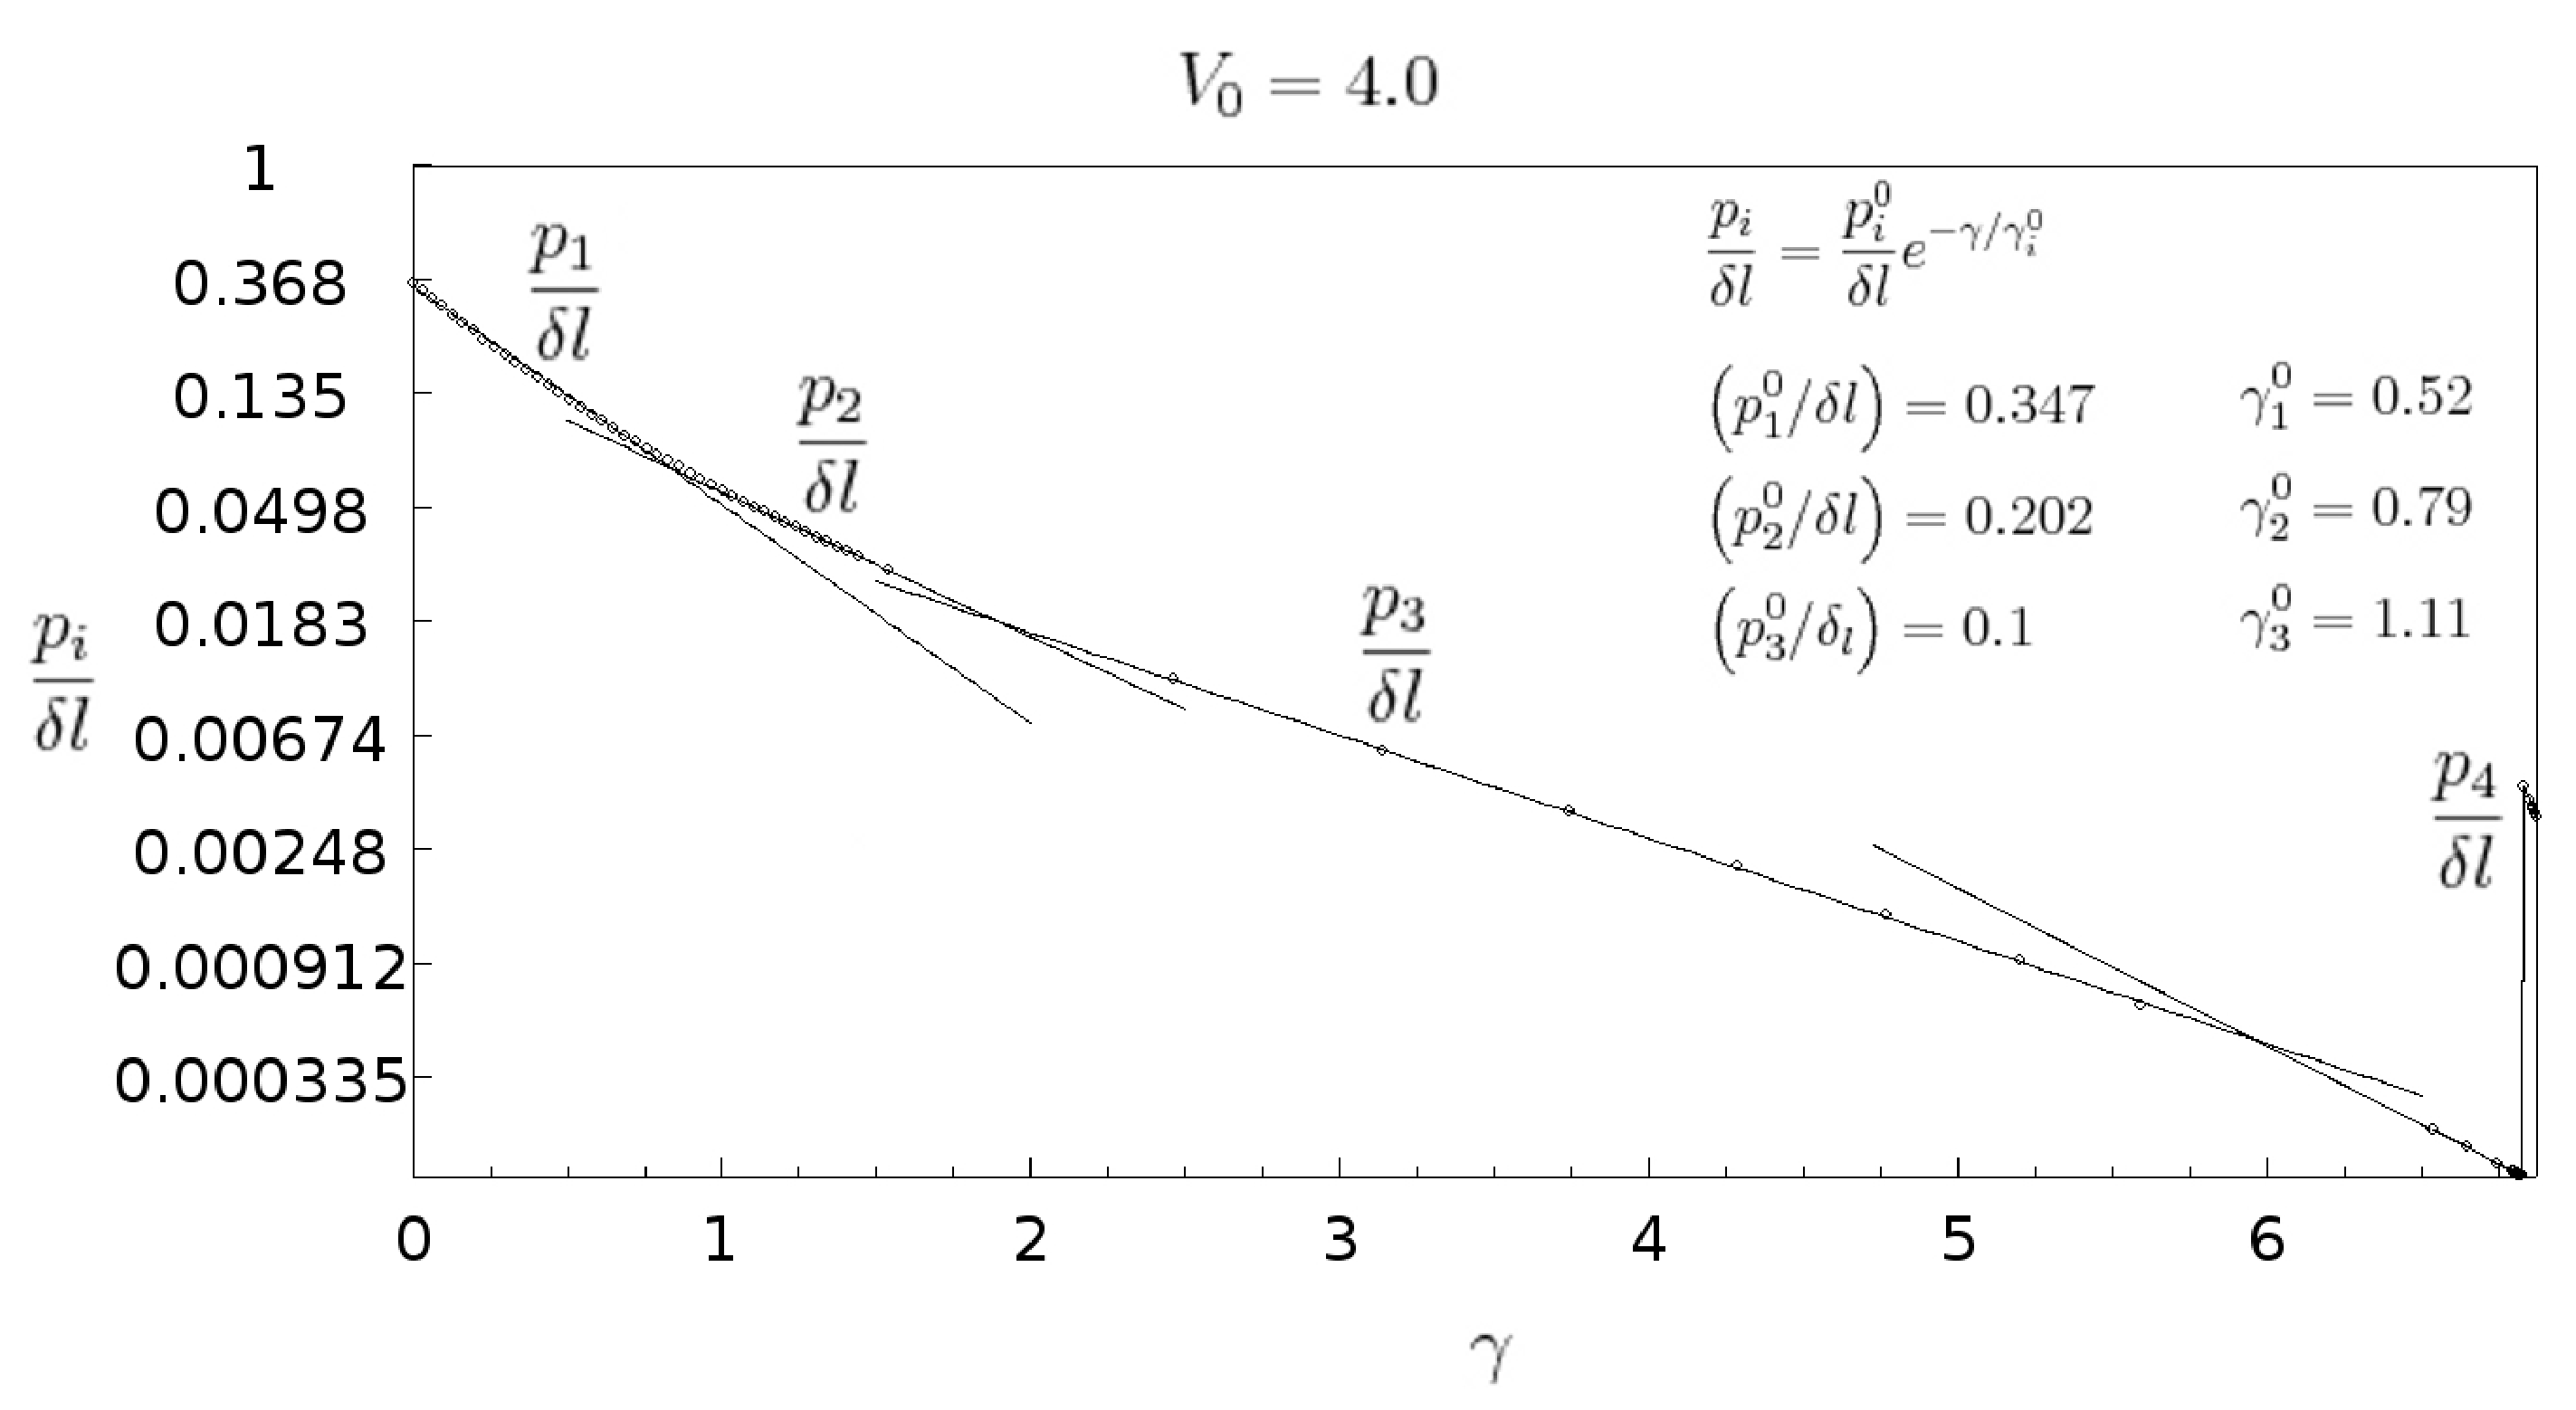
\psfig{file=jpegs/chapter-tof/fig2.eps,height=3.8in,width=5.7in}
\caption{Semi-logarithmic plot of the one dimensional probability density $p_i/{\delta l}$ of two particles being within a rectangular strip of arbitrarily small width $\delta l$ along the line $x_1=x_2$. $p_i/{\delta l}$ is plotted as a function of the strongly interacting parameter $\gamma$ for a constant $V_0=4.0$. The decay rate of the probability $p_i$ changes sharply at 4 regions, labeled by the index $i$. The data points (indicated by circles) have been fitted to exponential decay rates at each region (indicated by lines).The legend provides the numerically fitted values of the decay rates $\gamma^0_i$. Note the discontinuous spike at $\gamma\sim 7$.}
\label{fig:tonksparam:appendixtof}
\end{figure}
Here, $i$ is an index distinguishing different regimes of interest in the $\gamma$-space. Also, $p_i$ is the total probability that the two particles will be together within a rectangular strip along the line $x_1=x_2$ and arbitrarily small width $\delta l$. As expected, it vanishes for large values of $\gamma$.

In this strongly interacting regime, the two particles have no probability of occupying the same position simultaneously. Thus, they act in a way that is similar to a Tonks gas~\cite{tonks:gas}.  The transition to this regime is not consistent, however. We note four distinct ranges of $\gamma$ for which the decay rates of 
$p_i/{\delta l}$  are different. In the first three ranges, $p_i$ seems to be decaying exponentially ie $\left( p_i/{\delta l}\right)=\left( p^0_i/{\delta l} \right) e^{-(\gamma/\gamma^0_i)}$ for $i=1,2,3$. The data points have been fitted to exponents by the use of numerical nonlinear least-squares algorithms.
The decay rate, characterized by $ \gamma^0_i $, decreases sharply at $\gamma\sim 1, 2$ and $6$. Near $\gamma\sim 7$, there is a sharp increase in $p_i$ after which it continues to decrease. If we neglect the probability if it falls below $1/e$ of the maximum, then the 'strongly interacting regime' is achieved beyond $\gamma\sim 0.4$. In our case, we have chosen a $\gamma$ of $5.20142$ for our strongly interacting regime, placing the system in region $3$ of Fig~\ref{fig:tonksparam:appendixtof}. The value of $\left(V_0,U_0\right)$ chosen is $\left(4.0, 40.0\right)$.

The second regime, henceforth referred to as the 'single particle regime', will consist of a weakly attractive system and the well-depth as seen in~\cite{mypaper}. Thus, the parameter values chosen are $\left(7.2912229, -1.0\right)$.The probability distributions of the ground state  $|E_1\rangle$, as well as the excited states  $|E_2\rangle$ and  $|E_4\rangle$, given by Eqn~\ref{eq:hamscale:appendixtof}  are shown in Figs~\ref{fig:wavefunctions_tonks:appendixtof}.a through \ref{fig:wavefunctions_tonks:appendixtof}.c for the strongly interacting regime. Note that, as expected, there is virtually no probability that $x_1=x_2$.
%Fig. 3
\begin{figure}
\ 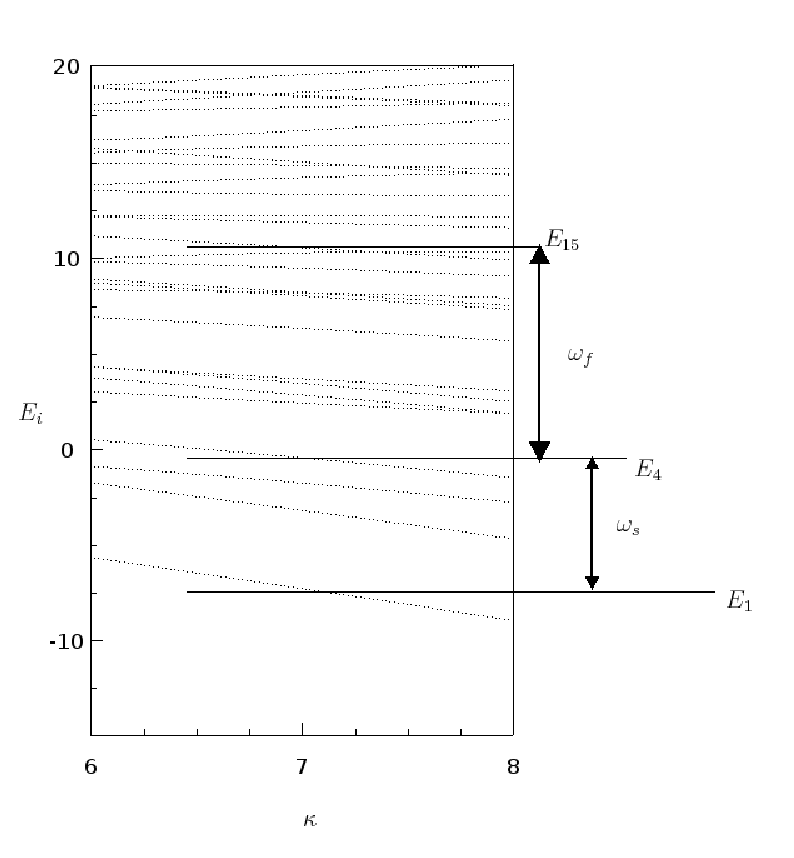
\psfig{file=jpegs/chapter-tof/fig3.eps,height=6.0in,width=3.0in}
\caption{Plots of energy eigenfunctions for the two interacting bosons in a double well potential in the strongly interacting regime. Figures (a) through (c) are contour plots of the probability density $|\langle x_1,x_2|E_1\rangle|^2$ ,  $|\langle x_1,x_2|E_2\rangle|^2$  and $|\langle x_1,x_2|E_4\rangle|^2$ respectively. The probabilities are plotted as functions of $x_1$ and $x_2$. All units for all figures are dimensionless}
\label{fig:wavefunctions_tonks:appendixtof}
\end{figure}
The probability distributions of the first seven quantum energy states of the system in the single particle regime are shown in Figs.~\ref{fig:wavefunctions:appendixtof}.a through  \ref{fig:wavefunctions:appendixtof}.g. Note the plots of the ground state, $|E_1\rangle$, third excited state, $|E_4\rangle$,  and sixth excited state $|E_7\rangle$. The dynamics of the system, when driven by sequential pulses whose energies are tuned to transitions between these states, show the effects of dynamical chaos through level-repulsion in the Floquet eigenphases~\cite{mypaper}. A crossing through the level-repelling region can be avoided if the radiation pulses are applied adiabatically, producing a chaos assisted passage as detailed in~\cite{mypaper}.
%Fig. 4
\begin{figure}
\ 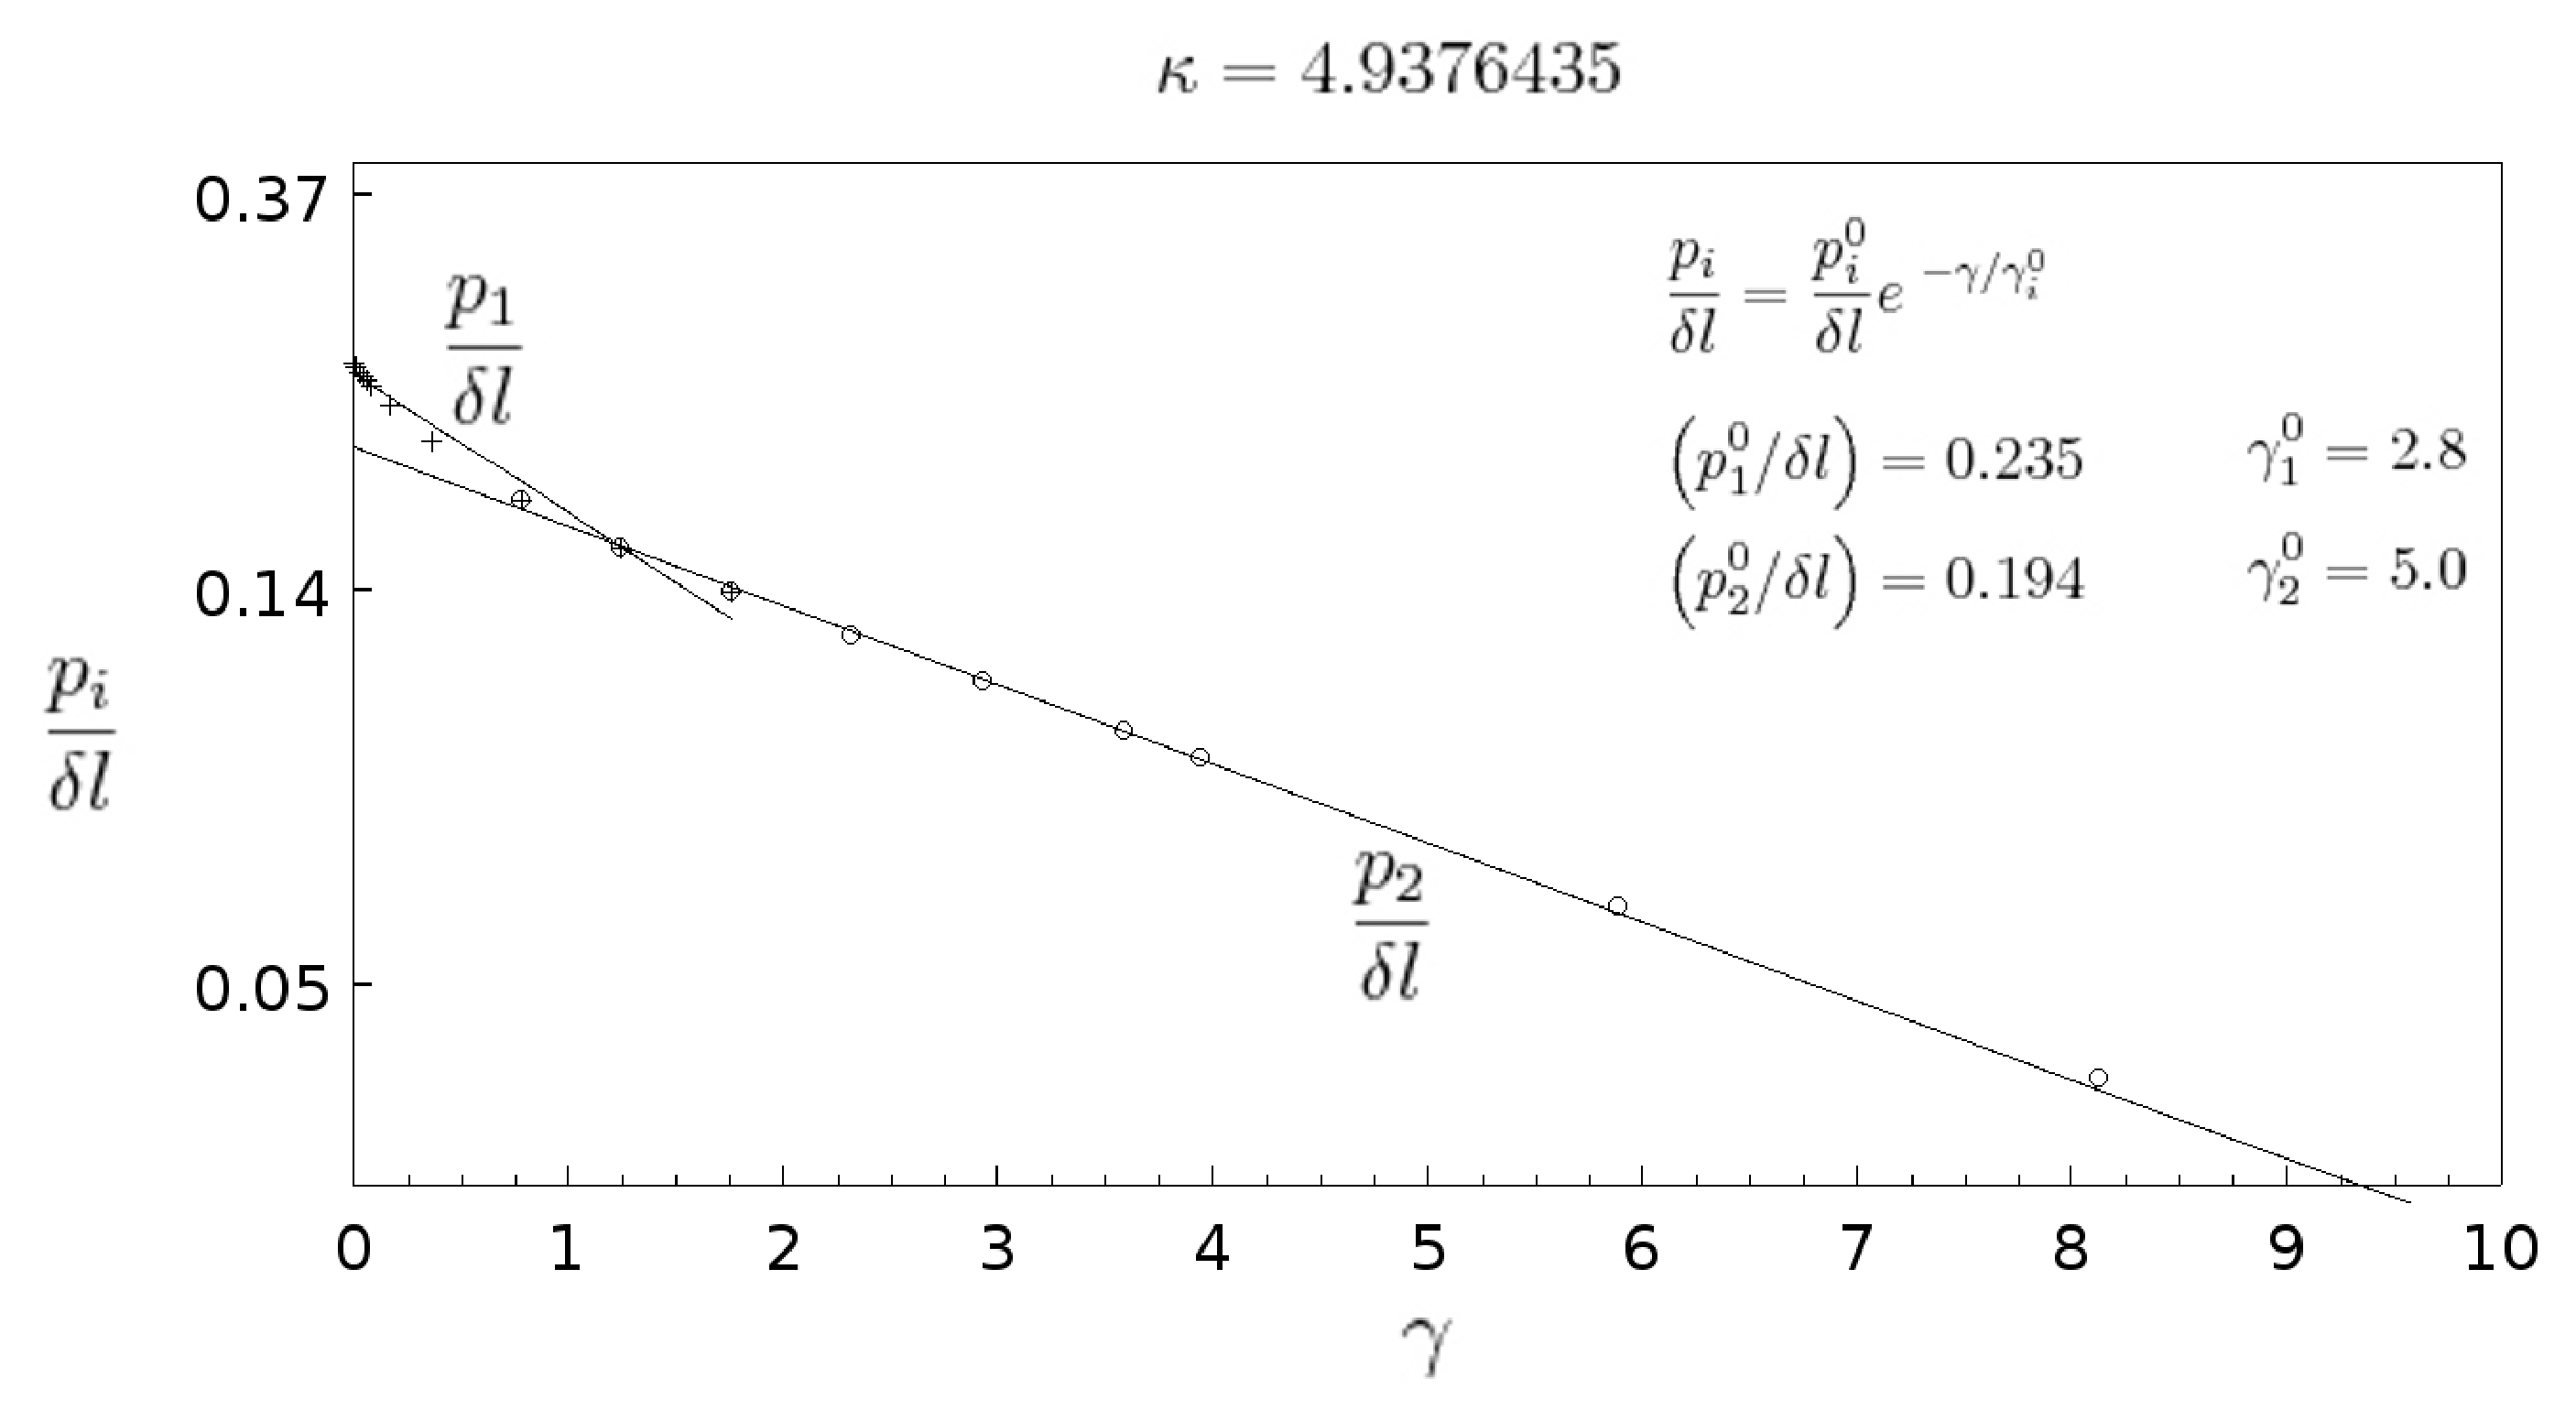
\psfig{file=jpegs/chapter-tof/fig4.eps,height=6.0in,width=4.0in}
\caption{Plots of energy eigenfunctions for the two interacting bosons in a double well potential in the single particle regime. All units are dimensionless. Figures (a) through (f) are contour plots of the probability density $|\langle x_1,x_2|E_1\rangle|^2$ through $|\langle x_1,x_2|E_6\rangle|^2$ respectively. Figure (g) is a contour plot of the probability density
$|\langle x_1,x_2|E_7\rangle|^2$.The peaks in the probability are numbered. The probabilities are plotted as functions of $x_1$ and $x_2$. All units for all figures are dimensionless}
\label{fig:wavefunctions:appendixtof}
\end{figure}
%
\section{\label{sec:2:appendixtof} Time of Flight Images} 
%
%
The normalized first order correlation function of a single double well is a measurement of the atomic density $n(x)$. Such correlations can be measured following a STIRAP transition by the time-of-flight (TOF) technique in which the trapped atoms are released sufficiently quickly  that the diabatic approximation in quantum mechanics can be applied. The atoms then expand ballistically until they reach a detection plate. If the plate is far enough from the double well system that the far-field approximation can be used, then the Green's Function for the system can be simplified and the time translation reduced to a simple Fourier Transform.  If the 'detector plane' coordinates are denoted by unprimed variables $\left[ x_1,x_2,t \right]$ and the double -well coordinates by primed variables $\left[ x'_1,x'_2,t \right]$ for a 2-particle system after all the external fields and traps have been diabatically switched off, and the interactions between the atoms rendered negligible by tuning a homogenous magnetic field close to the Feshbac resonance that adds an attractive amplitude to the normally repulsive point contact pseudopotential~\cite{feshbach:resonance}~\cite{pethick:bec}. The system then evolves ballistically in free space. 

The Green's Function or Propagator $G({\bf x},t;{\bf x}',t')$ is defined by
\begin{equation}
\Psi ({\bf x},t) = \int d^2x \mbox{ } G({\bf x},t;{\bf x}',t') \Psi ({\bf x}',t'),
\label{eq:greensfunction:appendix}
\end{equation}
where ${\bf x} = \left[ x_1, x_2 \right]$, and $\Psi({\bf x},t)$ is the wavefunction, with similar expressions for the primed coordinates. For free space, the relevant 1-dimensional Schr\"odinger equation for 2-particles is
\begin{eqnarray}
\left[ H-i\frac{\partial}{\partial t} \right] \Psi({\bf x},t) =0, \nonumber \\
H=-\left[ \frac{\partial^2}{\partial x^2_1} + \frac{\partial^2}{\partial x^2_2} \right].
\end{eqnarray}
 Thus, the Green's function~\cite{sakurai} will be the solution to
 \begin{equation}
 \left[ H-i\frac{\partial}{\partial t} \right] G({\bf x},t;{\bf x}',t') = \delta ({\bf x}-{\bf x}') \delta (t-t').
 \label{eq:greens:appendix}
 \end{equation}
The solution to Eqn~\ref{eq:greens:appendix} in free space is
\begin{equation}
G({\bf x},t;{\bf x}',t') = \frac{\sqrt{-i}}{L} \exp{\left[ i\pi | \frac{{\bf x}-{\bf x}'}{L}|^2 \right]}.
\label{eq:greensfn:appendix}
\end{equation}
Here, the ballistic de-Broglie equation,
\begin{equation}
L^2=4 \pi \tau,
\label{eq:debroglie:appendixtof}
\end{equation}
 provides the relation between the detector-system separation $L$ and the time-of-flight $\tau=\left(t-t'\right)$.

Now, consider such a two particle system localized at a site $j$. The wavefunction is localized about ${\bf x}'_j = \left[ x'_j, x'_j \right]$ and can be written in the form $\Psi({\bf x}'-{\bf x}'_j)$. We now use Eqns~\ref{eq:greensfn:appendix} and~\ref{eq:debroglie:appendixtof} on Eqn~\ref{eq:greensfunction:appendix}, and apply the shift theorem for Fourier transforms~\cite{goodman}~\cite{Grondalski:etal} to get
\begin{equation}
\Psi(x,\tau) = \sqrt{\frac{-i}{4\pi\tau}}\exp{\left[ i\frac{1}{2\tau}\left( \frac{|{\bf x}|^2}{2} + {\bf x}\bullet {\bf x}'_j\right)\right]} F\left[ \Psi({\bf x}')\right]_{{\bf u}=\frac{{\bf x}}{4\pi\tau}},
\label{eq:TOF:appendixtof}
\end{equation}
where the primed coordinates refer to the double well system, the unprimed coordinates refer to the detector, and $ F\left[ \Psi({\bf x}')\right]_{\bf u}$ is the Fourier transform
\begin{equation}
F\left[ \Psi({\bf x}')\right]_{\bf u} \equiv \frac{1}{2 \pi} \int d^2x' \Psi({\bf x}') e^{i{\bf u}\bullet{\bf x}'}.
\label{eq:ft:appendix}
\end{equation}
In the equation above,  ${\bf u} = \left[ u_1, u_2 \right]$ is the momentum space vector. For a large collection of such systems, each in the desired pure state, the measured TOF is simply the probability obtained from Eqn~\ref{eq:TOF:appendixtof} times the number of such double wells $N$ (which we shall subsequently drop off as an appropriately adjusted overall normalization).
\begin{equation}
n({\bf x})= N \frac{1}{4\pi\tau} | F\left[ \Psi({\bf x}') \right]_{{\bf u}=\frac{{\bf x}}{4\pi\tau}} |^2.
\label{eq:TOFmeas:appendixtof}
\end{equation}

We note that there are noticeable differences in the symmetries of the two states $|E_4\rangle$ and $|E_7\rangle$ (refer to Figs~\ref{fig:wavefunctions:appendixtof}). The distinctly resolved peaks in each wavefunction (labeled $1$ through $8$ for $|E_7\rangle$) can be approximated by elliptical Gaussian functions. Thus, the wavefunction can be represented by  a two-dimensional function as follows:
\begin{equation}
\Psi(x'_1, x'_2) = \sum_{i=1}^{R} {a_i}G\left( x'_1, x^i_1, \alpha^i_1\right) G\left( x'_2, x^i_2, \alpha^i_2\right),
\label{eq:gaussianfits:appendixtof}
\end{equation}
where
\begin{equation}
G(x,x^i,\alpha) =\left( \frac{2\alpha}{\pi}\right)^{1/4} e^{-\alpha \left(x-x^i \right)^2}.
\end{equation}
Here, $R$ is the number of peaks (8 for $|E_7\rangle$). Also,  we have rotated our coordinate system to the axes of symmetry (by $45$ degrees) of $|E_7\rangle$. Using the well-known relation for the Fourier transform of a Gaussian applied to Eqns~\ref{eq:TOFmeas:appendixtof} and~\ref{eq:gaussianfits:appendixtof}, we get (sans any overall normalizations), 
\begin{equation}
n(x_1,x_2) = | \sum_{j=1}^{R} a_j \left(\frac{1}{4\pi^2 \alpha^j_1\alpha^j_2}  \right)^{1/4} e^{i\frac{x_1x^j_1 + x_2x^j_2}{4\pi\tau}} e^{-\frac{x^2_1}{16\pi^2 \alpha^j_1\tau^2}} e^{-\frac{x^2_2}{16\pi^2 \alpha^j_2\tau^2}} |^2.
\label{eq:gaussianfitsexpand:appendixtof}
\end{equation}
We rewrite this as 
\begin{eqnarray}
n(x_1,x_2)=| \sum_{j=1}^R r_j(x_1,x_2) e^{i k_j x_1} |^2, \nonumber \\
r_j(x_1,x_2)=a_j \left( \frac{1}{4\pi^2\alpha^j_1\alpha^j_2} \right)^{1/4} e^{i\frac{x_2 x^j_2}{4\pi\tau}} e^{-\frac{x^2_1}{16\pi^2\alpha^j_1\tau^2}} e^{-\frac{x^2_2}{16\pi^2\alpha^j_2\tau^2}}, \nonumber \\
k_j = \frac{ x^j_1}{4\pi\tau}.
\label{eq:rthetasplit:appendixtof}
\end{eqnarray}
The expression above can be simplified to 
\begin{equation}
n(x_1,x_2)=\sum_{j=1}^{R}|r_j(x_1,x_2)|^2 + \sum_{\left\langle i,j \right\rangle} 2r^*_i(x_1,x_2) r_j(x_1,x_2) |\cos{(k_j-k_i)x}|.
\end{equation}
In order to get the density functional $n(x)$, we integrate out the $x_2$ (symmetries guarantee that the result will be the same if we integrate $x_1$ instead) and get
\begin{eqnarray}
n(x)=\sum_{j=1}^{R}r^2_j(x) + \sum_{\left\langle i,j \right\rangle} 2r^2_{ij}(x) |\cos{(k_j-k_i)x}|,
\label{eq:interesting:appendixtof}
\end{eqnarray}
where $\left\langle i,j \right\rangle$ are distinct (ie $i \neq j$) combination pairs of peaks. In the equation above, integrating $x_2$ by Gaussian integral methods leaves out a Gaussian dependencies in $x$ of $r_j$ and $r_{ij}$ (the subscripts for $x$ have been dropped). Thus,
\begin{eqnarray}
r^2_j(x) = \tau a^2_j \sqrt{\frac{4\pi}{\alpha^j_1}}  e^{-\frac{x^2}{16\pi^2\alpha^j_1\tau^2}}, \nonumber \\
r^2_{ij}(x)=2 \tau a_i a_j \left(\frac{1}{ \alpha^i_1 \alpha^j_1 \alpha^i_2 \alpha^j_2} \right)^\frac{1}{4} \sqrt{\pi\alpha^{ij}_2} e^{-\frac{\alpha^{ij}_2(x^j_2-x^i_2)^2}{4}} e^{-\frac{x^2}{16 \pi^2 \alpha^{ij}_1\tau^2}},
\end{eqnarray}
where we have defined
\begin{equation}
\frac{1}{\alpha^{ij}}\equiv \frac{1}{\alpha^i}+\frac{1}{\alpha^j}.
\end{equation}

From the plot of $|E_7\rangle$ for the single particle regime (see Fig~\ref{fig:wavefunctions:appendixtof}), we notice that there are only three distinct kinds of peaks (labeled $1$, $5$ and $8$). Thus there are three pairs whose $k$'s are unequal viz. $\left\langle 1,5 \right\rangle$ and $\left\langle 1,8 \right\rangle$ and $\left\langle 5,8 \right\rangle$. All other terms are absorbed into the perfect square terms in Eqn~\ref{eq:interesting:appendixtof}. Each such term is a Gaussian centered at $x=0$ with varying widths. If we look at values of $x$ sufficiently far from the center of the detector plate, those terms drop off quickly, leaving just the three oscillatory terms. This signal will be distinct from that obtained from the TOF of state $|E_4\rangle$, which has only $2$ such term (only $2$ distinct kinds of peaks). If the time-of-flight $\tau$ is chosen so that the values of $k_j-k_i$ are small, then the signal will look like an amplitude modulated sinusoid. 

\section{\label{sec:3:appendixtof} Time-of-Flight: Numerical Plots}
This section will detail the procedure for obtaining numerical plots of the tof distributions of the eigenstates of the double well system. The two boson problem in a double well is diagonalized as detailed in section~\ref{chapter-dblwell:diaghamilt} of chapter~\ref{chapter-dblwell}, and appendix~\ref{appendix-matelements}. Thus, the eigenfunctions are obtained as linear superpositions of the eigenfunctions of two bosons in a box of appropriately chosen length $L$, ie
\begin{eqnarray}
{\langle}x_1,x_2\vert n_1,n_2{\rangle} ^{(s)}=\frac{1}{\sqrt{2(1+\delta_{n_1,n_2})}} 
[{\langle}x_1|n_1\rangle{\langle}x_2|n_2\rangle +{\langle}x_1|n_2\rangle{\langle}x_2|n_1\rangle ], \nonumber \\
\langle x|n\rangle=\frac{1}{\sqrt{L}} \sin{\biggl[}{\frac{n\pi}{2}(\frac{x}{L}-1){\biggr]}},
\label{eq:pboxfn:appendix}
\end{eqnarray}
 if $|x_i|<L$, and $0$ otherwise. Thus, the final solution to an eigenfunction $|E_n\rangle$ of the double well will be a linear superposition of the  'finite wave train'  functions defined above, ie
\begin{equation}
\langle x_1,x_2|E_n\rangle =  \sum_{\left[n_1,n_2\right]=\left[1,1\right]}^{\left[ N,N \right]} C^{\left[n_1,n_2 \right]}_{E_j} {\langle}x_1,x_2\vert n_1,n_2{\rangle} ^{(s)},
\end{equation}
where the $C^{\left[n_1,n_2 \right]}_{E_j}$ are obtained numerically using the nonadaptive finite element method. This result can then be substituted into Eqn~\ref{eq:TOFmeas:appendixtof} to get
\begin{equation}
n(x_1,x_2) = N \frac{1}{4\pi\tau} |\sum_{\left[n_1,n_2\right]=\left[1,1\right]}^{\left[ N,N \right]} C^{\left[n_1,n_2 \right]}_{E_j} F\left[ {\langle}x'_1,x'_2\vert n_1,n_2{\rangle} ^{(s)} \right]_{\left[u_1,u_2\right]=\frac{\left[ x_1,x_2 \right]}{4\pi\tau}}|^2.
\label{eq:density:appendix}
\end{equation}
Using the linearity of Fourier Transforms and Eqn~\ref{eq:pboxfn:appendix}, we get
\begin{multline}
F\left[ {\langle}x'_1,x'_2\vert n_1,n_2{\rangle} ^{(s)} \right]_{\bf u}=\frac{1}{\sqrt{2(1+\delta_{n_1,n_2})}}\\
\left( F[{\langle}x_1|n_1\rangle]_{u_1} F[{\langle}x_2|n_2\rangle]_{u_2} +F[{\langle}x_1|n_2\rangle]_{u_1} F[{\langle}x_2|n_1\rangle]_{u_2}  \right).
\label{eq:ft:appendix}
\end{multline}
The Fourier transform of the finite wave train ($\langle x|n\rangle$ in Eqn~\ref{eq:pboxfn:appendix}) can be calculated using Gaussian integrations~\cite{arfken} to yield
\begin{equation}
F[\langle x' | n \rangle]_u = \frac{1}{\sqrt{2L\pi}}  \frac{1}{\left( \frac{n^2 \pi^2}{4 L^2}-u^2 \right) } \left[ 2u \sin{\frac{n \pi}{2}}-\frac{n \pi}{L} \sin{L u} \right],
\label{eq:pboxft:appendixtof}
\end{equation}
where $u$ is the momentum space vector. Thus, by plugging Eqn~\ref{eq:pboxft:appendixtof} into Eqn~\ref{eq:ft:appendix}, and that into Eqn~\ref{eq:density:appendix}, the tof distribution $n(x_1,x_2)$ can be obtained, the final density distribution is the density functional average of this result viz.
\begin{equation}
n(x)=\int dx' n(x, x').
\end{equation}
Thus, a numerical expression for Eqn~\ref{eq:TOFmeas:appendixtof} was obtained for two degrees of freedom $x_1$ and $x_2$, and the density functional $n(x)$ determined by integrating out one of the coordinates by adaptive Gauss-Kronrod quadrature. 

Numerical results for the tof distributions of the eigenstates of the double well for the strongly interacting and single particle regimes are shown in Figs~\ref{fig:tof_1lakh_tonks:appendixtof} and ~\ref{fig:tof_1lakh:appendixtof} respectively. The distributions are shown for tof $\tau=10^5$ units of $T_u$. All the dynamics is essentially independent of the characteristic length scale $L_u$ (the actual position of the well minima). For practical reasons, we choose an $L_u$ of $50$ $nm$~\cite{mypaper}. Consequently, with a Rubidium-85 atomic mass of $85.4678$ $g·mol^{-1}$, we get a $T_u$ of about $6.7$  $\mu s$, which makes $\tau$ to be $0.67$ seconds. Using Eqn~\ref{eq:debroglie:appendixtof}, we get a detector distance of about $2.2$ $cm$. 

Figures~\ref{fig:tof_1lakh_tonks:appendixtof}(a) through (c) show the tof distributions of the states $| E_1\rangle$, $| E_2\rangle$, and $| E_4\rangle$ respectively for the strongly interacting gas detailed in section 1. Note that the the momentum distribution of $| E_1\rangle$, closely approximates the Heavyside function that is characteristic of the momentum distribution of a Tonks gas~\cite{tonks:gas} (barring the lack of any occupancy at zero momentum, which is forbidden in this case due to a nonzero value of the ground state energy $E_1$).

Figures~\ref{fig:tof_1lakh:appendixtof}(a) through (c) show the tof distributions of the states $| E_1\rangle$, $| E_4\rangle$, and $| E_7\rangle$ respectively in the single particle regime detailed in section 1.Note that, as predicted by the calculations in section~\ref{sec:2}, the number of distinct oscillations in each distribution correspond to the number of distinct pairs of peaks seen in the wavefunctions. Thus, each state generates a particular signature in the tof. Since the transitions to $|E_4\rangle$   and $|E_7\rangle$ are caused by crossing or avoiding a chaos assisted adiabatic passage, the amplitude modulation in the tof differentiates between the two outcomes. In case there is an incoherent excitation, there will be large numbers of overlapping or closely spaced peaks and the oscillations will constructively interfere everywhere, thus distinguishing the resultant signal from one obtained by the TOF of a coherent excitation. Thus,  the influence (or lack thereof) of chaos in the underlying classical dynamics can be indirectly inferred by the one extra oscillation in Fig~\ref{fig:tof_1lakh:appendixtof}(c) compared to Fig~\ref{fig:tof_1lakh:appendixtof}(b).

Time of flight fluorescence methods for profiling the wavefunction, such as measuring the momentum distribution by interrupting the particle flow with counter-propagating laser beams and then measuring fluorescence as a function of time (time of flight absorption)~\cite{fluorescense}~\cite{fluorescense:web}, will have high signal to noise ratio (compared to absorption)~\cite{raizen}.  Single shot fluorescence images should duplicate the profile shown in Figs~\ref{fig:tof_1lakh:appendixtof}(a)-(c) for a double well system produced by optical lattices. For a single magnetically confined double well, repeated measurements of position by the means of atom detectors, or by performing scanning tunneling microscopy on an appropriate substrate where the atoms are allowed to deposit after their tof expansion, should reproduce the required results.
\pagebreak
%Fig 1 (repeat from previous chapter)
%\begin{figure} 
%\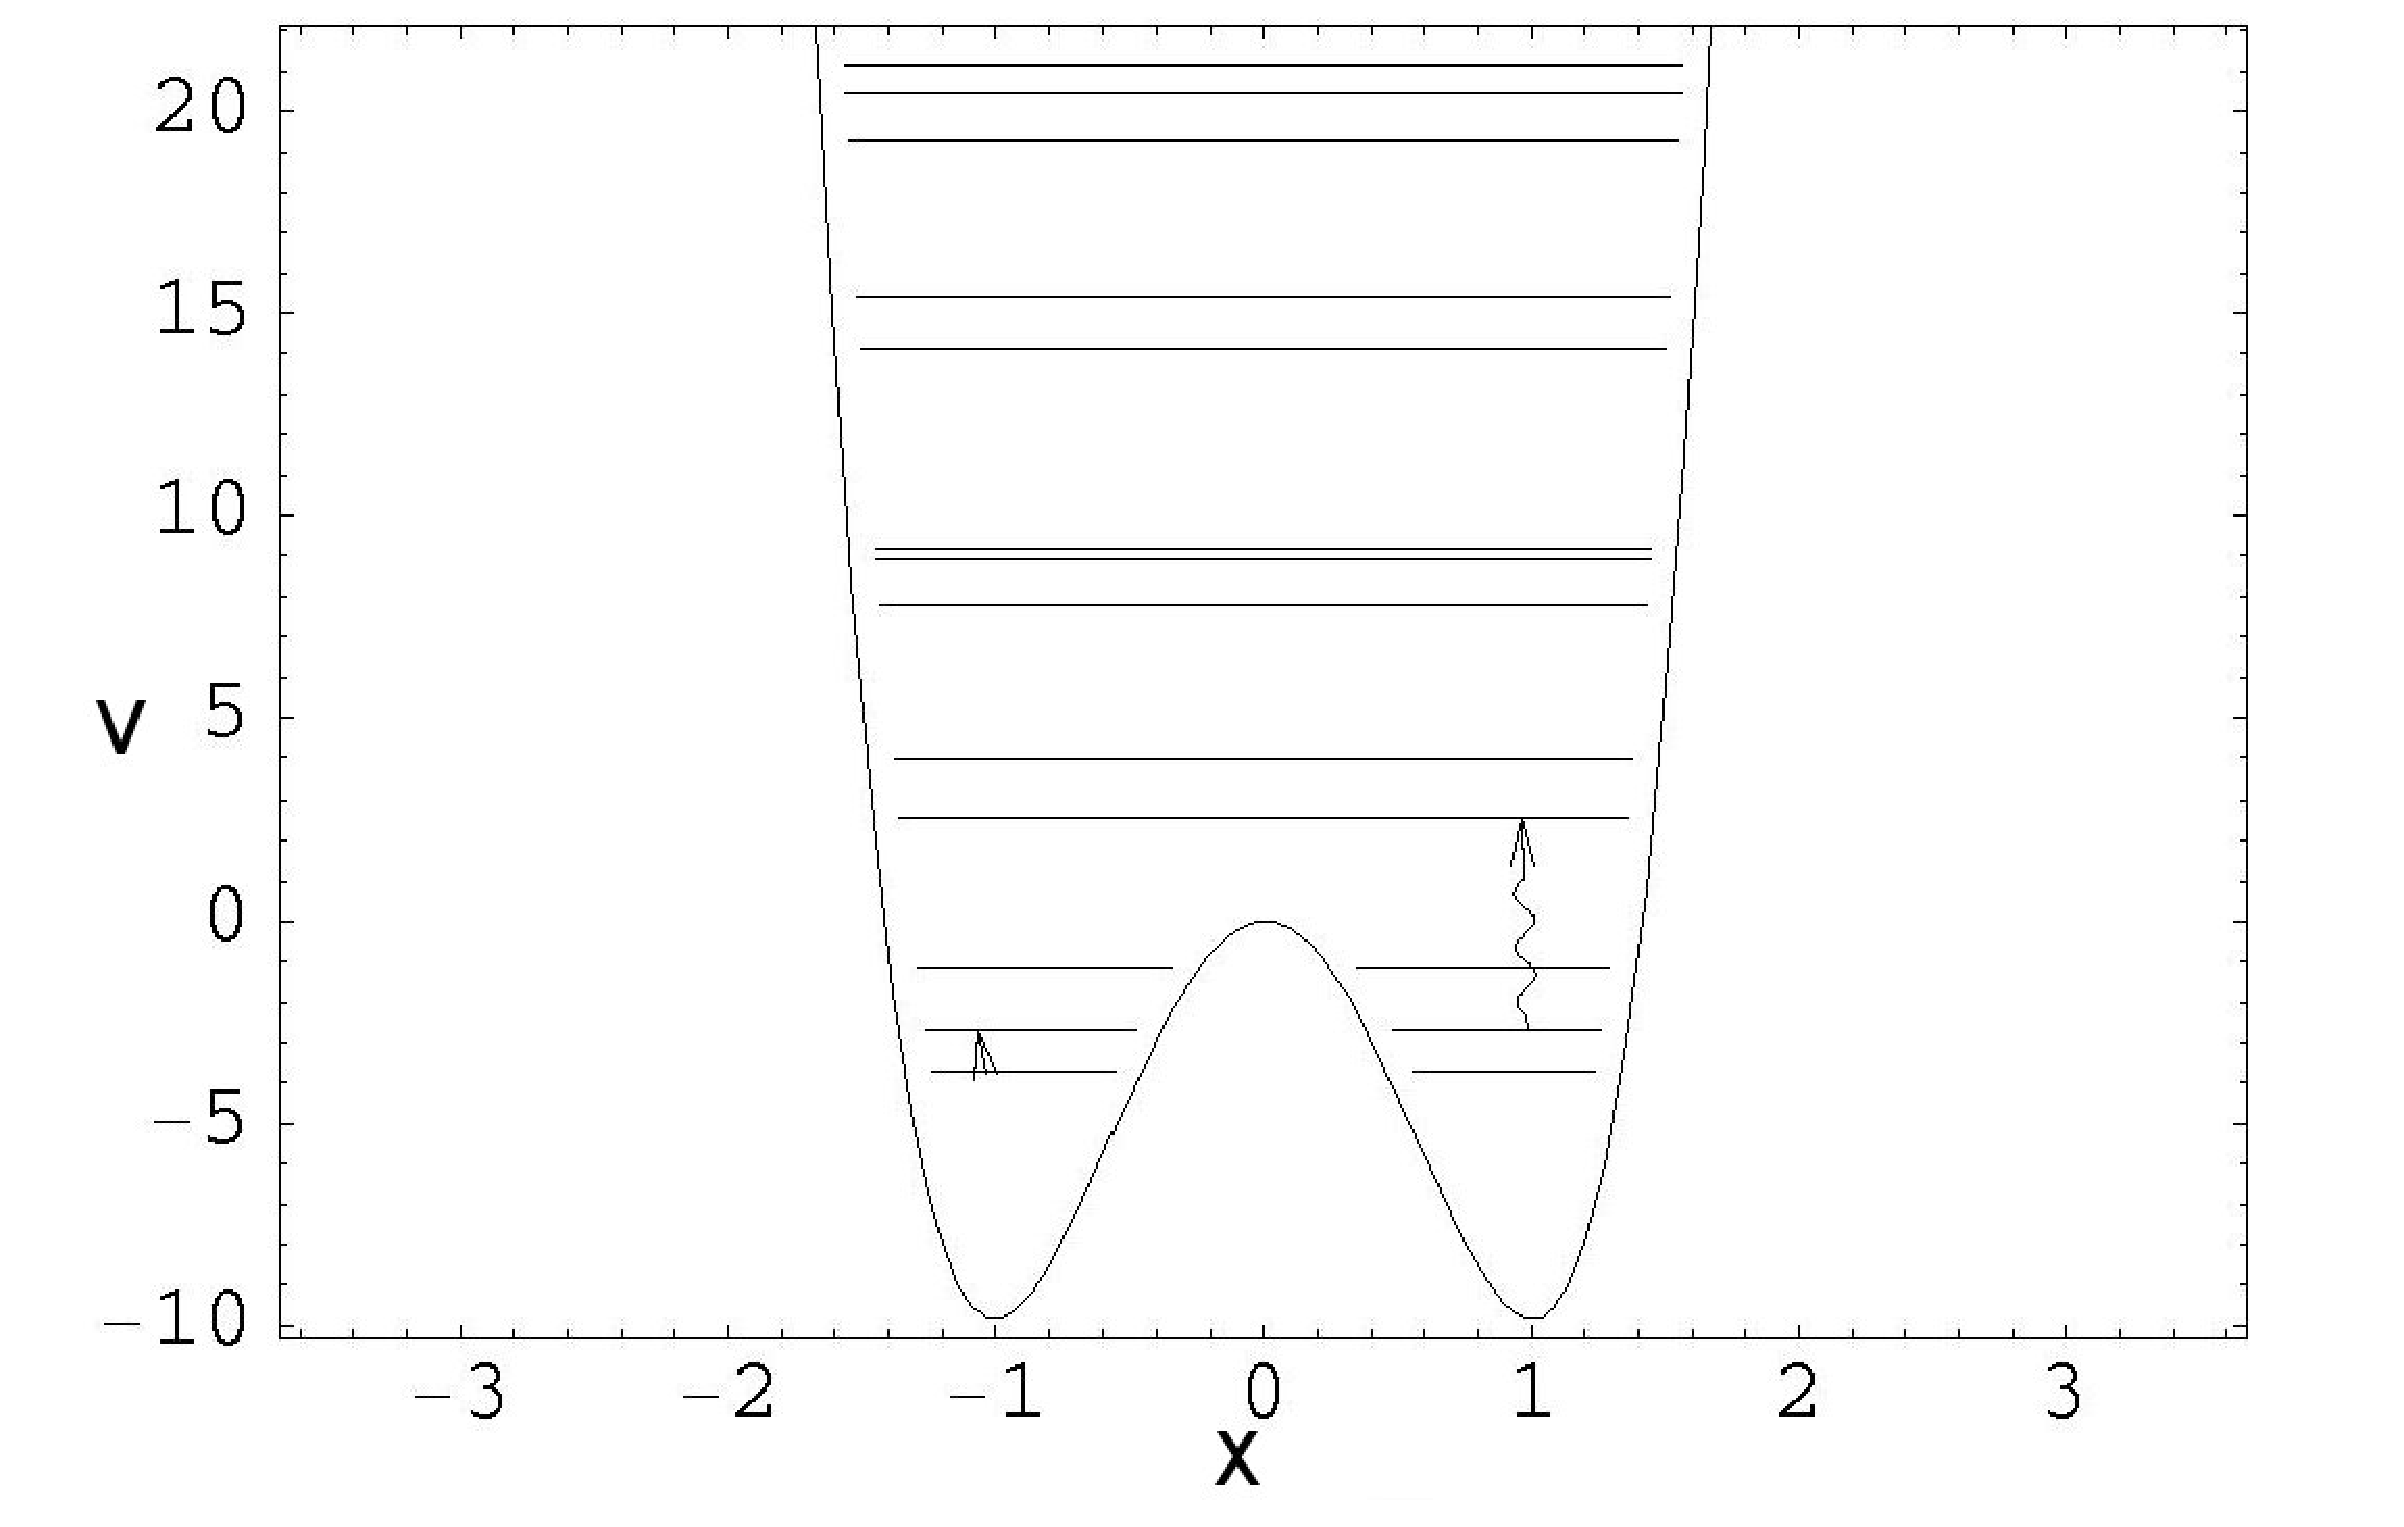
\psfig{file=jpegs/chapter-tof/fig1.eps,height=3.0in,width=5.0in}
%\caption{Plot of the double-well potential experienced by each boson in case 2. The energy levels, $E_1=-6.42262$, $E_2=-5.68883$ and $E_4=0.640055$  of the interacting two-boson system (interaction strength  $U_0=-1.0$) are also sketched, with wavy arrows denoting the levels connected by the STIRAP pulses. Note the slightly detuned resonance between the $2 \leftrightarrow 4$ and the $4 \leftrightarrow 7$ levels where $E_7=6.96998$. Here, $V_0=7.2912229$.}
%\label{fig:doublewell_case02}
%\end{figure}

%Fig. 5
\begin{figure}
\ 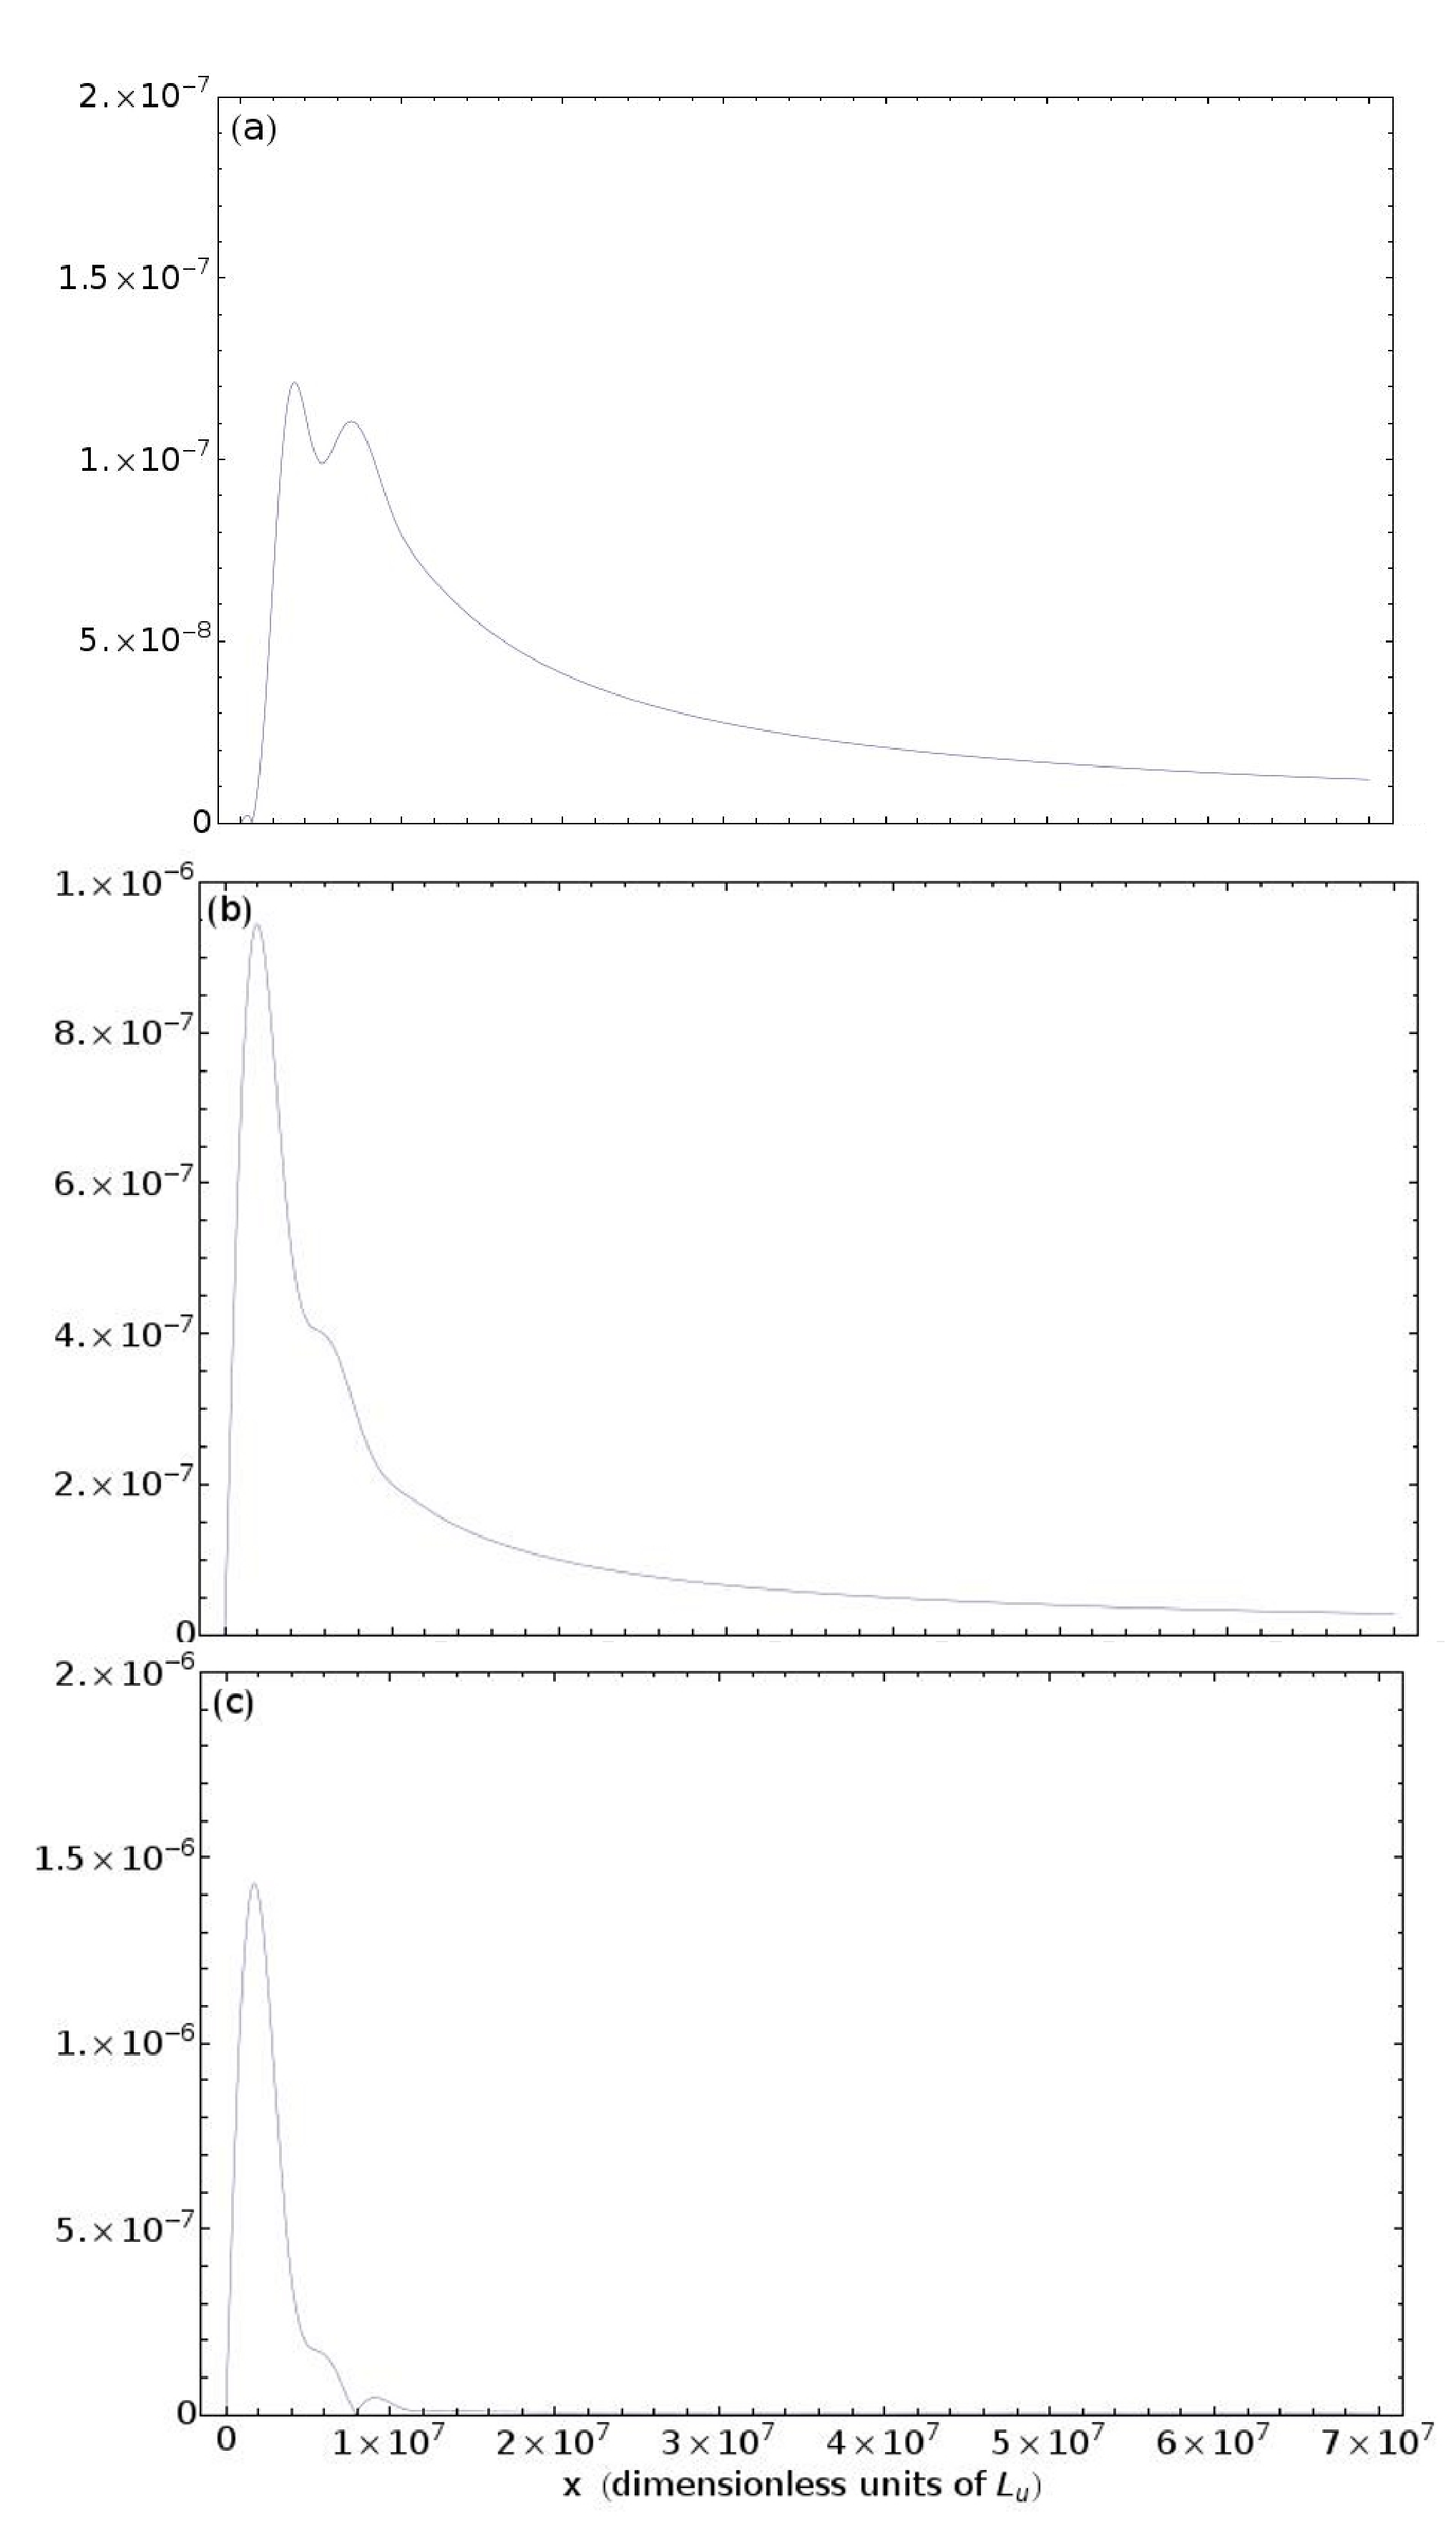
\psfig{file=jpegs/chapter-tof/fig5.eps,height=6.0in,width=4.0in}
\caption{Figures (a) through (c) are plots of the one-dimensional time-of-flight distributions for the double-well eigenstates $| E_1\rangle$, $| E_4\rangle$ and $| E_7\rangle$ respectively in the strongly interacting regime. The distributions are symmetric about $x=0$, so only the positive half is shown. The number density $n(x)$ in the ordinate is for $10^6$ double wells after a time of flight $\tau = 10^5$ (in units of $T_u$). The abscissa is shown in dimensionless units of $L_u$. }
\label{fig:tof_1lakh_tonks:appendixtof}
\end{figure}

%Fig. 6
\begin{figure}
\ 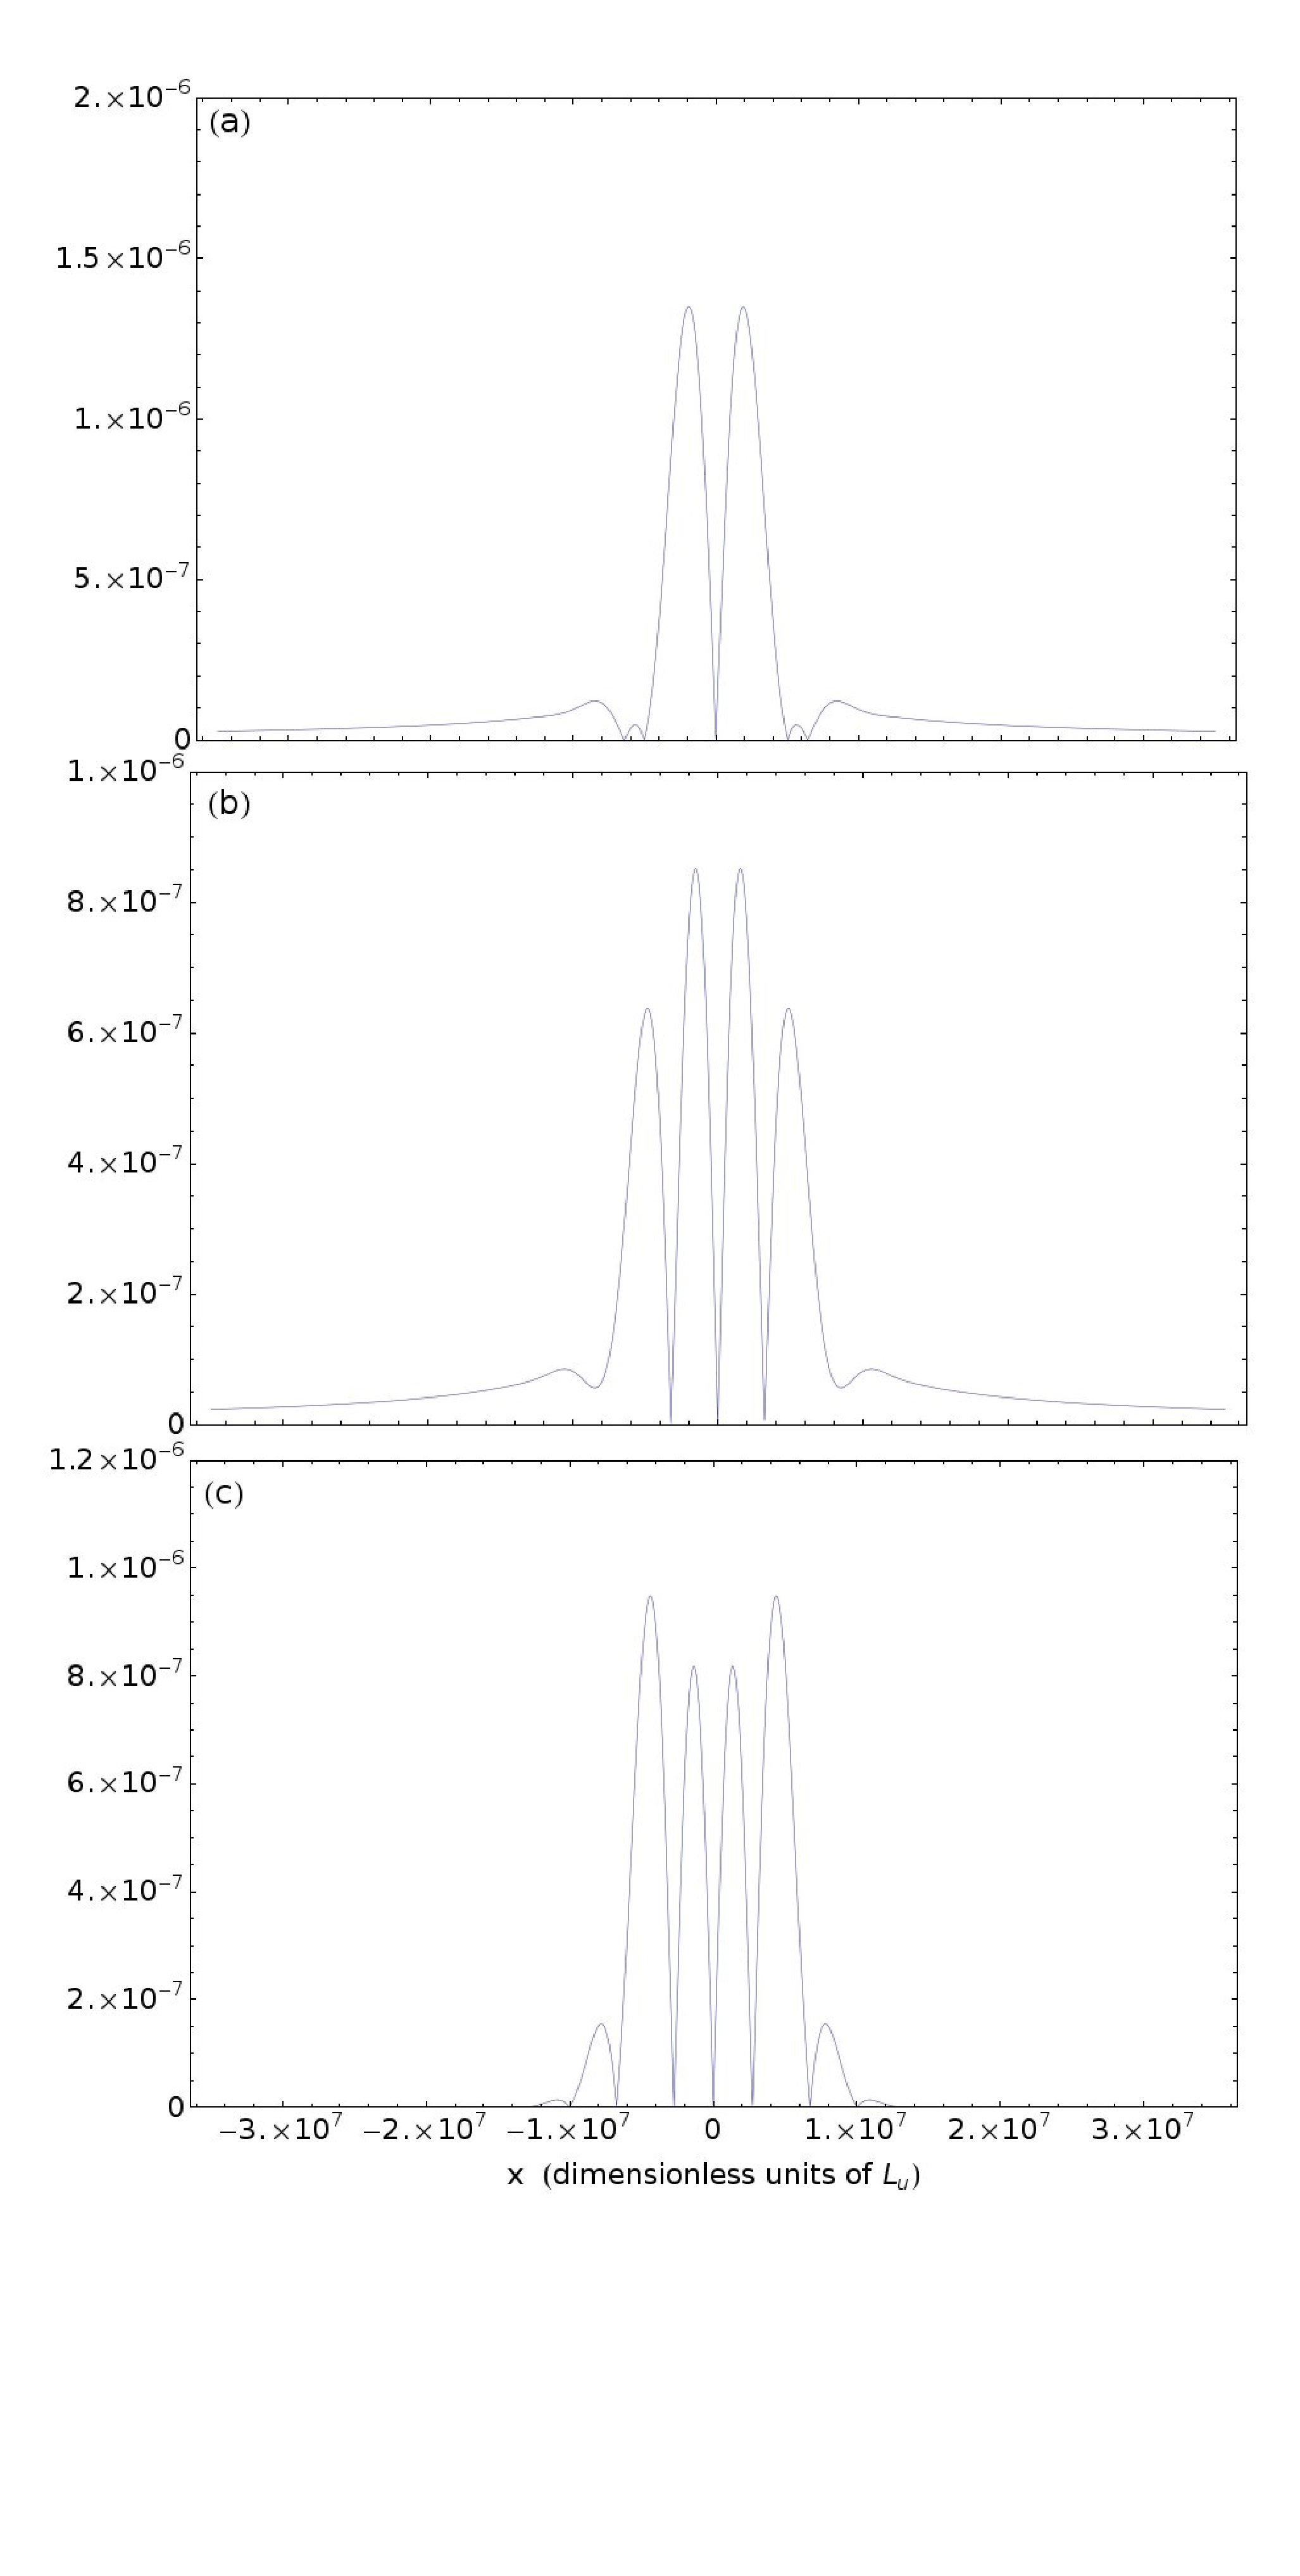
\psfig{file=jpegs/chapter-tof/fig6.eps,height=6.0in,width=4.0in}
\caption{Figures (a) through (c) are plots of the time-of-flight distributions for the double-well eigenstates $| E_1\rangle$, $| E_4\rangle$ and $| E_7\rangle$ respectively in the single particle regime. The number density $n(x)$ in the ordinate is for $10^6$ double wells after a time of flight $\tau = 10^5$ (in units of $T_u$). The abscissa is shown in dimensionless units of $L_u$.}
\label{fig:tof_1lakh:appendixtof}
\end{figure}
